\begin{figure}
    \centering
    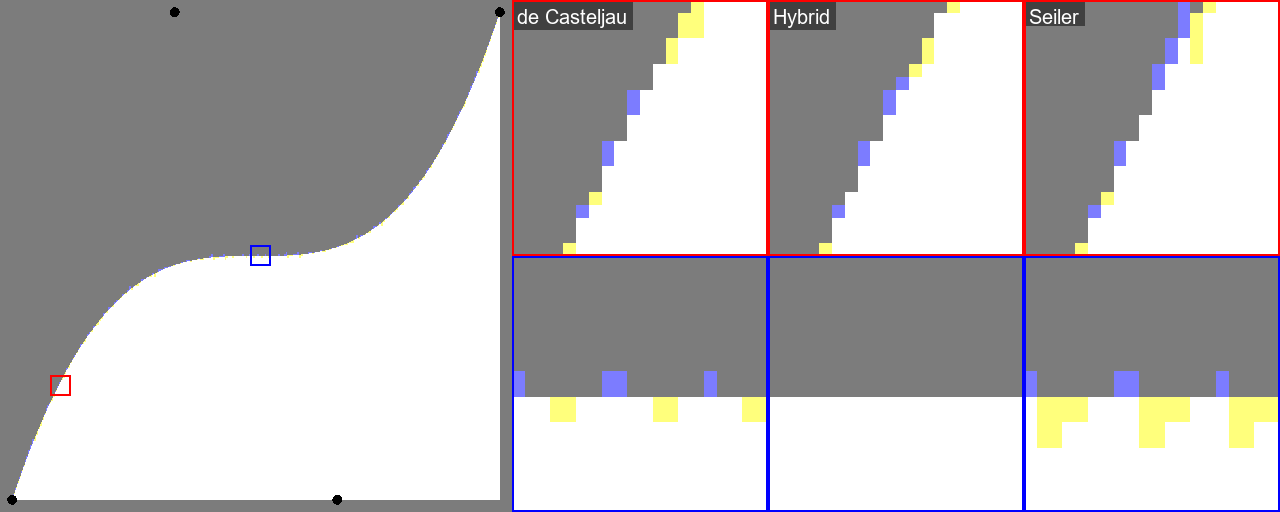
\includegraphics[width=\textwidth]{Diagrams/CurveAccuracy/diagram.png}
    \caption{Using the texture interpolator to evaluate Bézier curves suffers from quantization errors due to fixed point quantization of the $(u,v)$ coordinates.
    Here a cubic curve is shown evaluated using the de Casteljau texture method which samples a 2x2x2 volume texture with a single texture read. A hybrid mode is shown
    which evaluates two quadratic curves with the texture interpolator and then does the final lerp in the shader at full 32 bit floating point precision to reduce the error.
    Lastly the Seiler method is shown which takes a single sample of a 2x2 texture. In all images, yellow is the ground truth evaluated as a polynomial in the shader, and blue is
    added in for the comparison curve to show the error. The full sized image shows the de Casteljau method compared to the ground truth.}
    \label{fig_curve_accuracy}
\end{figure}
